\documentclass{article}
\usepackage{graphicx} % Required for inserting images
\usepackage[a4paper,margin=3cm]{geometry}
\usepackage{CJKutf8}
\usepackage{indentfirst}
\usepackage{subfigure}

\title{问题求解与实践课程大作业2测试说明}
\author{邴乙恒 522031910191}
\date{December 2023}

\begin{document}
\begin{CJK}{UTF8}{gbsn}

\maketitle

\section{开始界面}

\begin{figure}[h]
    \centering
    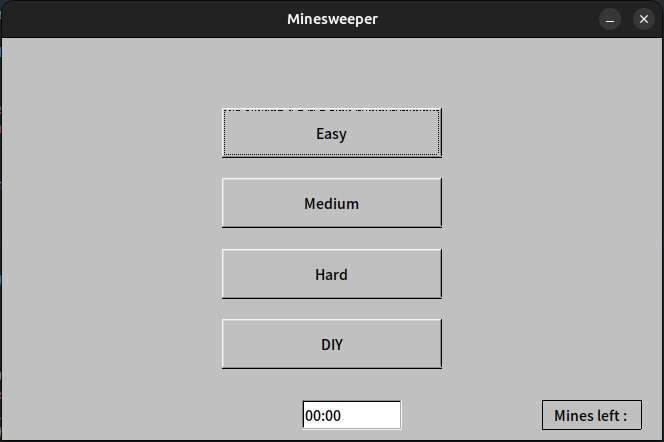
\includegraphics[width=0.6\textwidth]{test1.jpg}
    \caption{游戏开始界面}
    \label{fig:example1}
\end{figure}

由图片我们可以看到,游戏开始界面包括了三个难度按钮以及一个自定义按钮。点击难度按钮可以选择游戏难度,点击自定义按钮可以自定义游戏难度。

玩家在进入游戏时会先看到这个开始界面,在一轮游戏结束后,玩家可以选择点击重置按钮重新开始游戏并重新选择难度,也可以看到这个界面。

\section{游戏界面}

\begin{figure}[h]
    \centering
    \subfigure[简单难度]{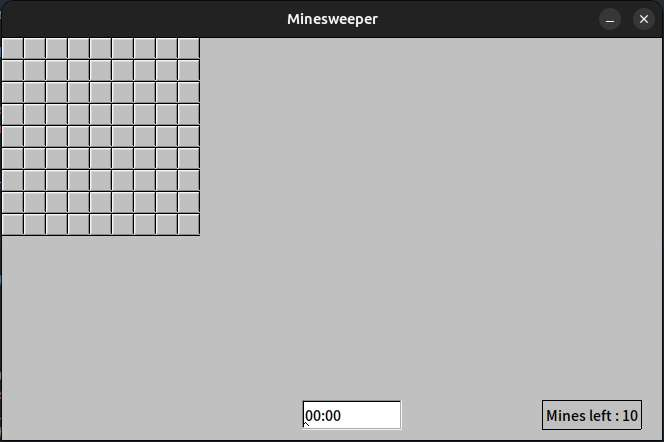
\includegraphics[width=0.3\textwidth]{test2.jpg}}
    \hspace{0.2cm}
    \subfigure[中等难度]{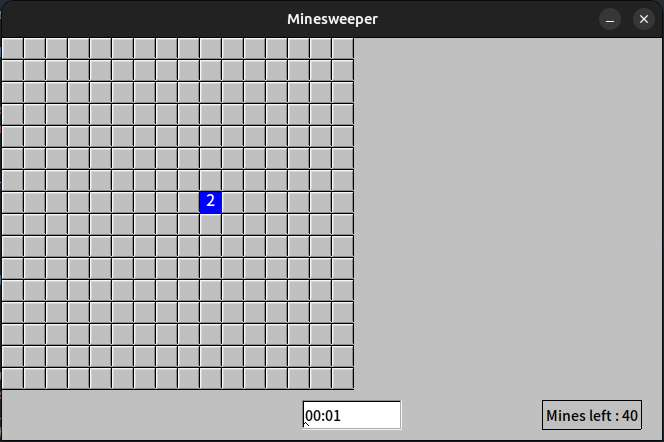
\includegraphics[width=0.3\textwidth]{test3.jpg}}
    \hspace{0.2cm}
    \subfigure[困难难度]{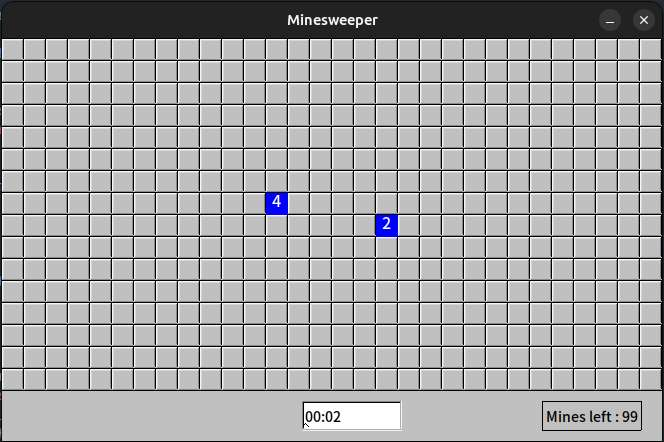
\includegraphics[width=0.3\textwidth]{test6.jpg}}
    \caption{各种难度游戏界面}
    \label{fig:example2}
\end{figure}

在玩家选择后,玩家会进入不同难度的游戏界面(包括自定义难度),之前选择难度使用的按钮将会隐藏以免影响玩家正常游戏。游戏界面包括了计时器、剩余地雷数量、重置按钮以及游戏格阵。各种难度的游戏界面如图所示。

\section{游戏结束界面}

\begin{figure}[h]
    \centering
    \subfigure[触雷画面]{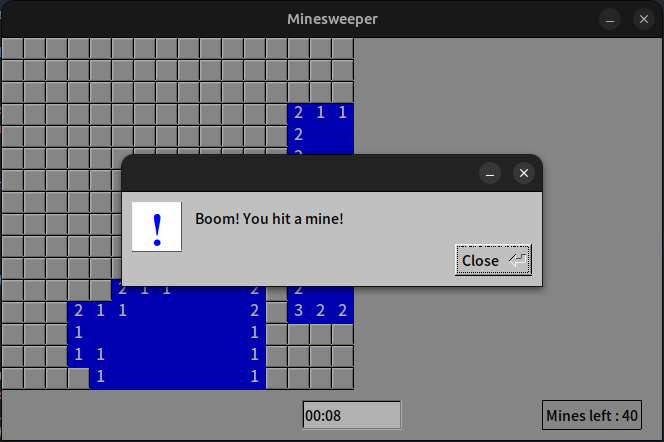
\includegraphics[width=0.3\textwidth]{test4.jpg}}
    \hspace{0.2cm}
    \subfigure[显示剩余地雷]{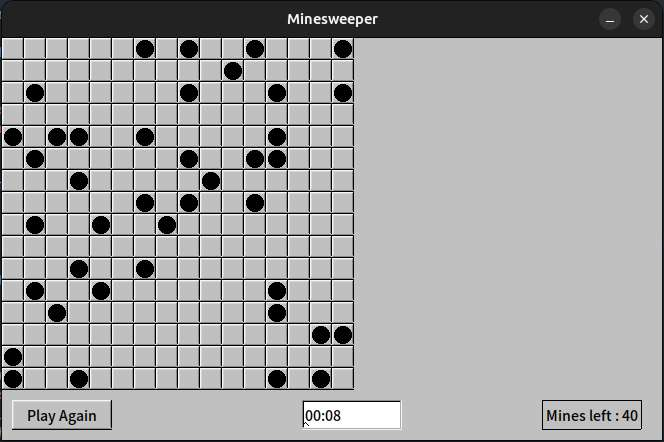
\includegraphics[width=0.3\textwidth]{test5.jpg}}
    \caption{失败界面}
    \label{fig:example3}
\end{figure}

\begin{figure}[h]
    \centering
    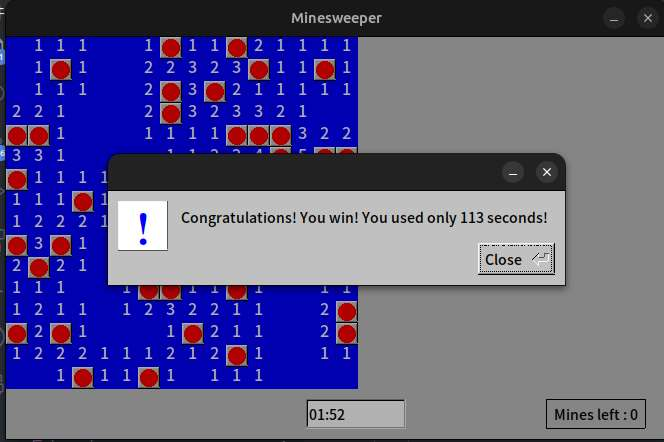
\includegraphics[width=0.4\textwidth]{test8.jpg}
    \caption{胜利界面}
    \label{fig:example4}
\end{figure}

在玩家失败触雷或者找到所有的地雷获得胜利后,这一轮游戏将结束,出现如图所示的结束画面。玩家可以选择点击重置按钮重新开始游戏并重新选择难度,也可以选择关闭窗口退出游戏。

\section{自定义界面}

\begin{figure}[h]
    \centering
    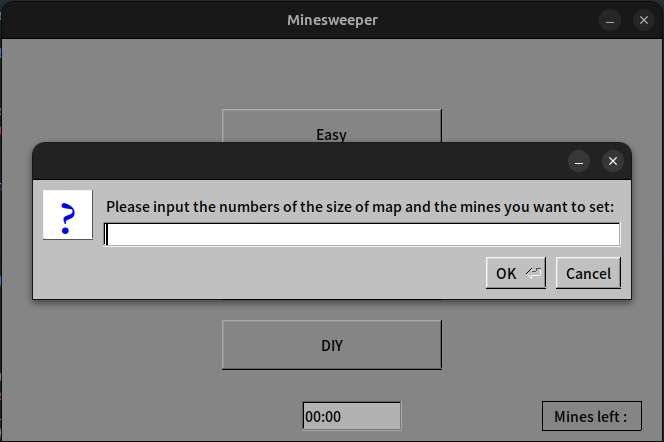
\includegraphics[width=0.6\textwidth]{test7.jpg}
    \caption{自定义界面}
    \label{fig:example5}
\end{figure}

另外,玩家在自定义游戏难度时可以看到如图所示的提示框,在框内输入用空格分开的三个数字表示格阵的宽度,高度以及雷的数目即可。如果输入不合法(如输入的不是数字或者输入的雷数比格子数多或者输入为0),则会弹出一个警告框提示玩家重新输入。





\end{CJK}
\end{document}